% !TeX root = ../04_C01_habermann_koester_rohde.tex

\begin{center}
    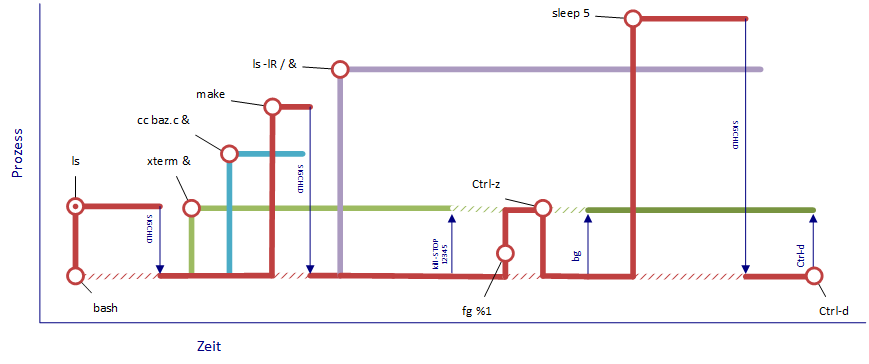
\includegraphics[width=\textwidth]{Sourcen/Aufgabe3.png}
\end{center}

Unsere Bash starten zuerst \C{ls} im Vordergrund und wartet auf dessen Terminierung.
Sobald \C{ls} terminiert, sendet es \m{SIGCHILD} an die bash, welche dadurch wieder aktiv läuft. \par\medskip

Das \C{xterm} wird im Hintergrund gestartet und läuft parallel zur bash. \newline
\C{cc baz.c \&} ist ein symbolic link, der auf einen symbolic link zeigt, der auf den \C{gcc}-Compiler zeigt.
Dieser führt also die Kompilierung im Hintergrund aus und terminiert dann. \par\medskip

\C{make} führt ein Makefile aus und beendet sich danach.
\C{bash} erhält hier wieder ein \m{SIGCHILD} und geht somit wieder ``in Betrieb''. \newline
\C{ls -lR / \&} wird wieder im Hintergrund ausgef\"{u}hrt und terminiert nach der Ausgabe des Root-Verzeichnisses.
Der Aufruf erfolgt hier rekursiv, wir gehen daher davon aus, dass es sehr lange dauert, bis der Prozess terminiert.
Daher haben wir hier mit einer Terminierung kurz vor Ende der Laufzeit ``gerechnet''. \par\medskip

Das Signal \m{STOP} wird über \C{kill -STOP 12345} an unsere imaginäre Prozess-ID von \C{xterm} gesendet, welches daraufhin angehalten wird.
\C{fg \%1} holt es wieder in den Vordergrund und führt es fort; \C{Ctrl-z} ist äquivalent zum vorherigen Signal.
Durch \C{bg} wird der Prozess, der nun im Hintergrund gestoppt ist, wieder angestossen.
Der Befehl \C{sleep 5} lässt die bash warten, bis die 5 Sekunden um sind, und sich \C{sleep} mit einem \m{SIGCHILD} abmeldet. \newline
Schließlich sendet \C{Ctrl-d} ein \m{End-of-File}-Signal, wodurch sich die \C{bash} und \C{xterm} beenden.
